% ============================================================
%  第二章 PID控制器
%  整理自《控制工程基础》读书笔记
%  说明：内容与读书笔记逐句对应，公式与表述保持不变。
% ============================================================

PID控制器是一种常用的反馈控制器，由比例项（\emph{proportional}）、积分项（\emph{integral}）和导数项（\emph{derivative}）组成，因此得名。

下面说明一些术语：
\begin{itemize}
	\item 基准（\emph{reference}）称为\textbf{设计点}（\emph{setpoint}）；
	\item 输出（\emph{output}）称为\emph{过程变量}（\emph{process variable}）或\emph{测量位置}（\emph{measured position}）。
\end{itemize}

然后误差写作
\begin{equation}
	e(t)=r(t)-y(t) .
	\label{eq:pid-error}
\end{equation}

下面将对关心的不同物理量应用比例控制器。这将对恒定和移动设定值的导数项的行为提供更完整的解释，这种直觉将延续到本书后面介绍的现代控制方法。

\begin{note}
	看完书能回答这个问题吗？
\end{note}

比例项将位置误差驱动为零，导数项将速度误差驱动为零，积分项累积速度误差为零，积分项累积设定点和输出曲线之间的面积（位置误差的积分），并将当前总和添加到控制输入。下面将对其中的每一个进行更详细的介绍。

\section{比例项（Proportional term）}
比例项使位置误差变为零。

\begin{figure}[htbp]
	\centering
	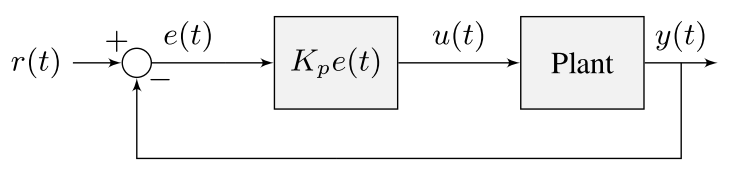
\includegraphics[width=0.6\textwidth]{Figure/比例控制器 1.png}
	\caption{比例控制器}
	\label{fig:p-controller}
\end{figure}

\begin{definition}[P控制器]
	\begin{equation}
		u(t)=K_{p}e(t) .
		\label{eq:p-controller}
	\end{equation}
	这里：
	\begin{itemize}
		\item $K_{p}$ 为比例增益；
		\item $e(t)$ 是当前时间 $t$ 的误差。
	\end{itemize}
\end{definition}

\begin{figure}[htbp]
	\centering
	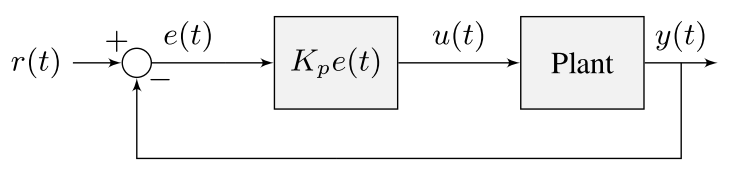
\includegraphics[width=0.6\textwidth]{Figure/比例控制器 1.png}
	\caption{比例控制器（续）}
	\label{fig:p-controller-2}
\end{figure}

比例增益就像一个可以被软件定义的弹簧（\emph{Software-defined springs}），把系统向目标的位置拽。

对比一下来理解一下：

力学里弹簧弹力满足
\begin{equation}
	F=k(r-x) .
	\label{eq:spring}
\end{equation}

这里的控制量 $u(t)$ 满足
\begin{equation}
	u(t)=K_{p}e(t)=K_{p}(r(t)-y(t)) .
	\label{eq:p-controller-spring}
\end{equation}

这样看来，比例控制器就像一根弹簧，初始位置在目标位置，不断地把系统的位置向目标位置拽，直到系统位置误差为 $0$。

\begin{note}
	想起来大二下学期一个寻常的周四下午，和张老师和刘方鑫师兄看师兄的毕业论文的时候，张老师画的图，原来是这样。恍如隔世。
\end{note}

\section{导数项（Derivative term）}
导数项使速度误差变为零。

\begin{definition}[PD控制器]
	\begin{equation}
		u(t)=K_{p}e(t)+K_{d}\frac{de}{dt} .
		\label{eq:pd-controller}
	\end{equation}
	这里：
	\begin{itemize}
		\item $K_{p}$ 是比例增益；
		\item $K_{d}$ 是导数增益。
	\end{itemize}
\end{definition}

\begin{figure}[htbp]
	\centering
	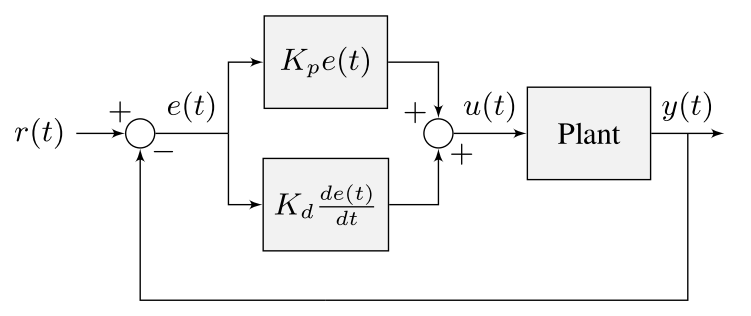
\includegraphics[width=0.6\textwidth]{Figure/PD控制器.png}
	\caption{PD控制器}
	\label{fig:pd-controller}
\end{figure}

可以看出一个PD控制器由两部分组成：
\begin{itemize}
	\item 一个对位置进行控制的P控制器；
	\item 一个对速度进行控制的P控制器。
\end{itemize}
速度设定点由位置设定点随时间变化的方式隐含地提供。

书上举了一个电梯的PD控制的例子：

\begin{figure}[htbp]
	\centering
	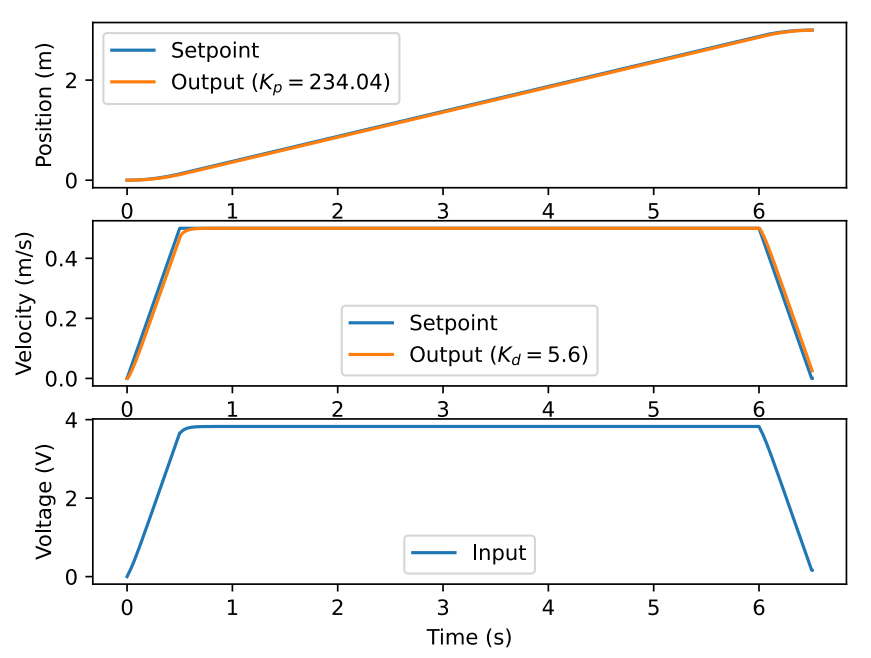
\includegraphics[width=0.7\textwidth]{Figure/电梯上的PD控制器.png}
	\caption{电梯上的PD控制器}
	\label{fig:pd-elevator}
\end{figure}

\begin{proof}[PD控制器就是两个P控制器的证明]
	第一步，对时间进行离散化处理，得
	\begin{equation}
		u_{k}=K_{p} e_{k}+K_{d} \frac{e_{k}-e_{k-1}}{\Delta t} .
		\label{eq:pd-proof-1}
	\end{equation}
	其中：
	\begin{itemize}
		\item $u_{k}$ 是时间步长 $k$ 处的控制输入；
		\item $e_{k}$ 是时间步 $k$ 处的误差；
		\item $\Delta t$ 是时间步长持续时间。
	\end{itemize}
	\begin{gather}
		u_k = K_p(r_k - y_k) + K_d \frac{(r_k - y_k) - (r_{k-1} - y_{k-1})}{\Delta t} , \label{eq:pd-proof-2} \\
		u_k = K_p(r_k - y_k) + K_d \frac{r_k - y_k - r_{k-1} + y_{k-1}}{\Delta t} , \label{eq:pd-proof-3} \\
		u_k = K_p(r_k - y_k) + K_{d} \left(\frac{r_k - r_{k-1} - y_k + y_{k-1}}{\Delta t}\right) , \label{eq:pd-proof-4} \\
		u_k = K_p(r_k - y_k) + K_d \left(\frac{(r_k - r_{k-1}) - (y_k - y_{k-1})}{\Delta t}\right) , \label{eq:pd-proof-5} \\
		u_k = K_p(r_k - y_k) + K_d \frac{(r_k - r_{k-1})}{\Delta t} - \frac{(y_k - y_{k-1})}{\Delta t} . \label{eq:pd-proof-6}
	\end{gather}
\end{proof}

如果设定点是恒定的，则隐含的速度设定点为零，因此，如果系统在运动，$K_d$ 项会减慢系统的速度。这就像一个“软件定义的阻尼器”。这种情况在闭门器上很常见，它们的阻尼力随速度线性增加。

\section{积分项（Integral term）}
积分项随时间累积设定点和输出曲线图之间的面积（即位置误差的积分），并将当前总和与控制输入相加。

\begin{definition}[PI控制器]
	\begin{equation}
		u(t)=K_{p}e(t)+K_{i}\int_{0}^{t} e(\tau)\,d\tau .
		\label{eq:pi-controller}
	\end{equation}
	积分从时间 $0$ 积分到当前时间 $t$。我们使用 $\tau$ 进行积分，因为我们需要一个变量在整个积分过程中接受多个值，但我们不能使用 $t$，因为我们已经将其定义为当前时间。
\end{definition}

下面是 PI 控制器的一个方框图：

\begin{figure}[htbp]
	\centering
	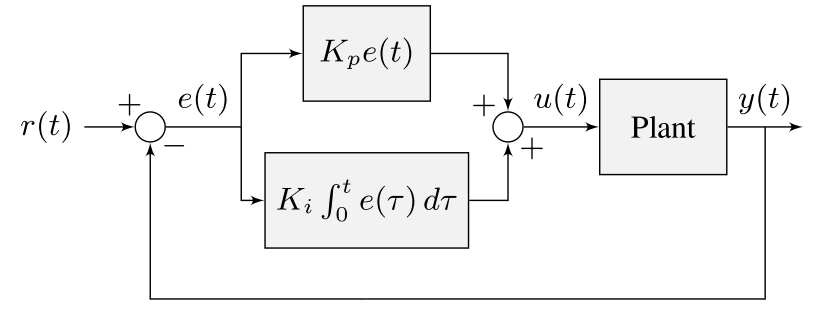
\includegraphics[width=0.6\textwidth]{Figure/PI控制器方框图.png}
	\caption{PI控制器方框图}
	\label{fig:pi-controller}
\end{figure}

当系统在稳态时接近设定值时，比例项可能太小，不能将输出一路拉到设定值，而导数项为零。这可能会导致稳态误差，如下图所示。

\begin{figure}[htbp]
	\centering
	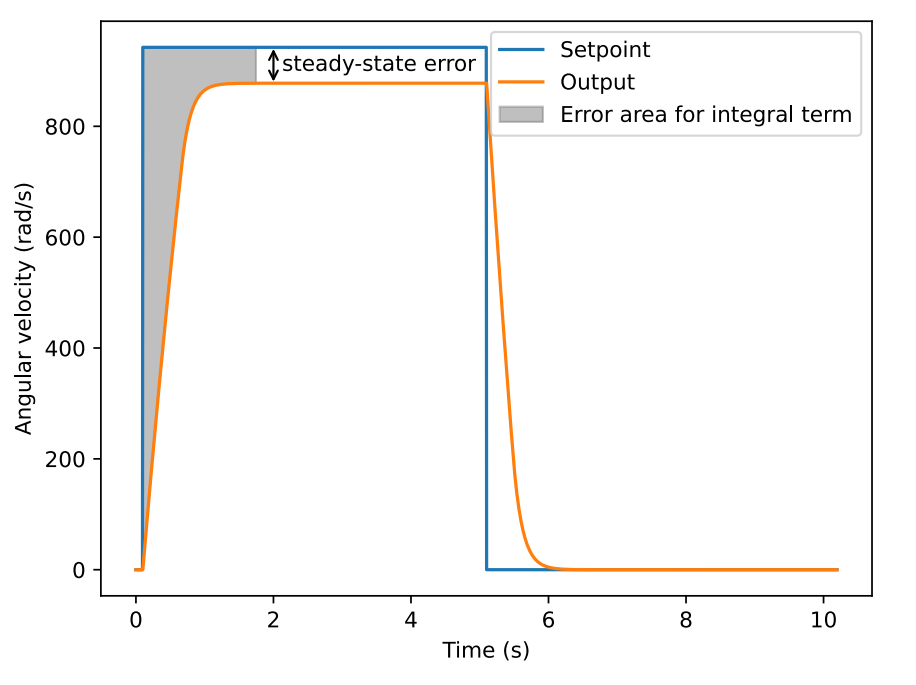
\includegraphics[width=0.6\textwidth]{Figure/具有稳态误差的飞轮上的P控制器.png}
	\caption{具有稳态误差的飞轮上的P控制器}
	\label{fig:p-steady-error}
\end{figure}

消除稳态误差的一种常见方法是对误差进行积分，并将其添加到控制输入。这增加了控制力，直到系统收敛。下图显示了添加到飞轮控制器中的积分器如何消除稳态误差。

\begin{figure}[htbp]
	\centering
	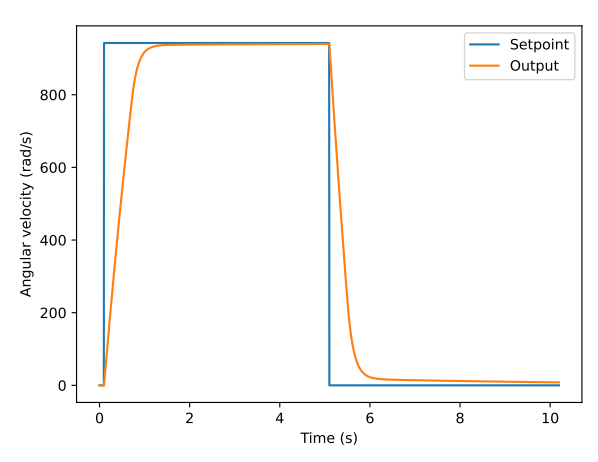
\includegraphics[width=0.6\textwidth]{Figure/无稳态误差的飞轮PI控制器.png}
	\caption{无稳态误差的飞轮PI控制器}
	\label{fig:pi-steady-error}
\end{figure}

然而，积分增益过高可能会导致超调，如下图所示。

\begin{figure}[htbp]
	\centering
	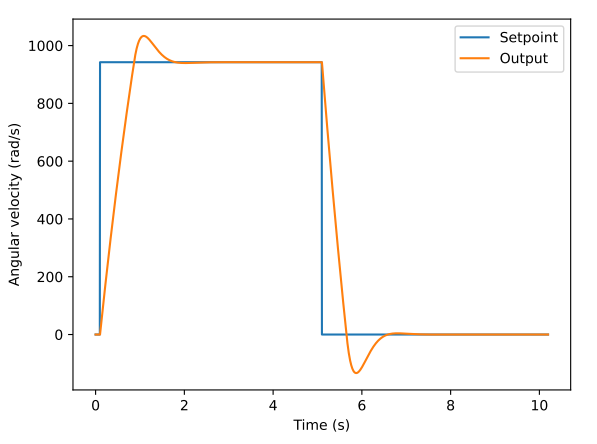
\includegraphics[width=0.6\textwidth]{Figure/大K_i增益超调飞轮的PI控制器.png}
	\caption{大 $K_i$ 增益超调飞轮的PI控制器}
	\label{fig:pi-overshoot}
\end{figure}

\section{PID控制器定义}
对比例项、导数项和积分项进行超级拼装，可得 PID 控制器。

\begin{definition}[PID控制器]
	\begin{equation}
		u(t)=K_{p} e(t)+K_{i} \int_{0}^{t} e(\tau) d \tau+K_{d} \frac{d e}{d t} .
		\label{eq:pid}
	\end{equation}
\end{definition}

\begin{figure}[htbp]
	\centering
	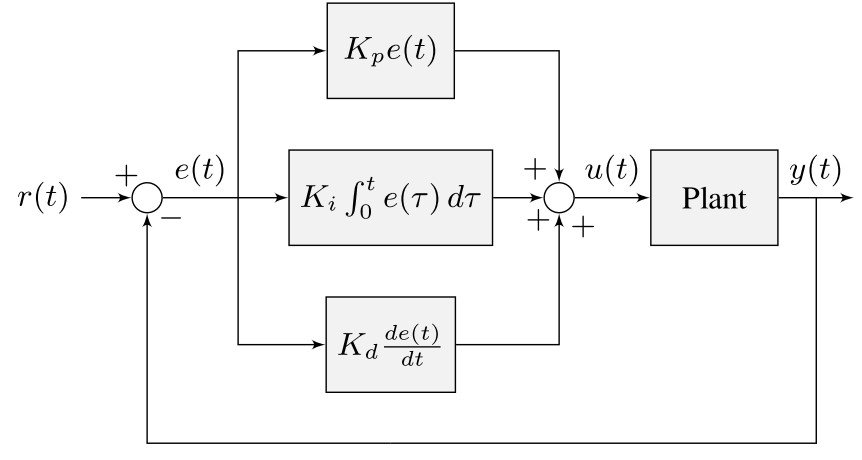
\includegraphics[width=0.6\textwidth]{Figure/PID控制器方框图.png}
	\caption{PID控制器方框图}
	\label{fig:pid-controller}
\end{figure}

\section{响应类型}
由 PID 控制器驱动的系统通常有三种类型的响应：\textbf{欠阻尼}（\emph{underdamped}）、\textbf{过阻尼}（\emph{overdamped}）和\textbf{临界阻尼}（\emph{critically damped}）。如下图所示。

\begin{figure}[htbp]
	\centering
	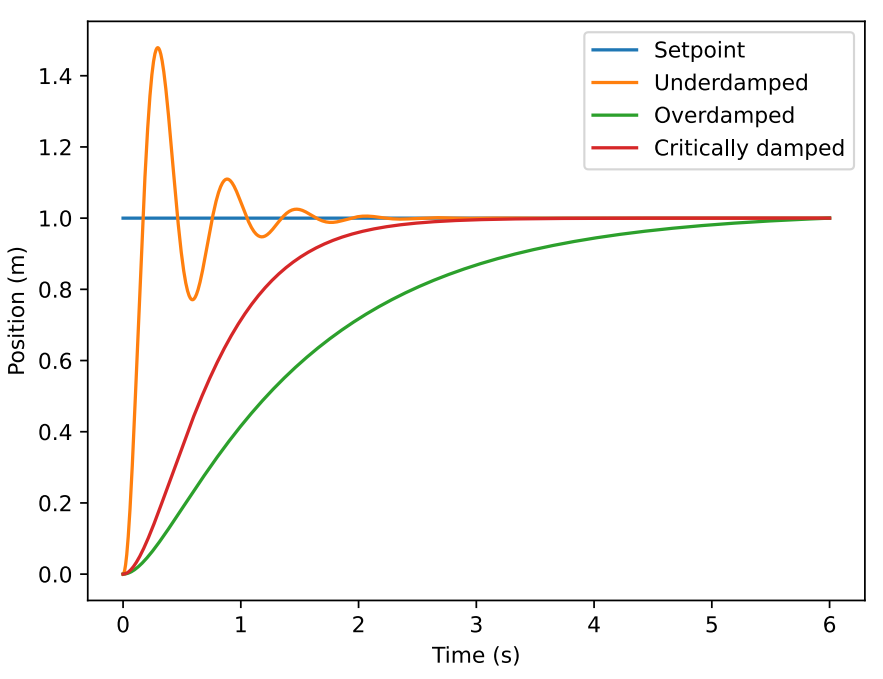
\includegraphics[width=0.85\textwidth]{Figure/PID控制器响应类型.png}
	\caption{PID控制器响应类型}
	\label{fig:pid-response}
\end{figure}

对于上图中的阶跃响应，上升时间是施加阶跃输入后系统初始达到基准所需的时间。稳定时间是系统在施加阶跃输入后稳定在基准上所花费的时间。

在达到设定点之前，欠阻尼响应围绕基准振荡。过阻尼的反应是缓慢上升的，并且不会超出参考范围。临界阻尼的响应具有最短的上升时间，而不会围绕基准振荡。

\section{手动调参}
这些步骤适用于位置 PID 控制器。速度 PID 控制器通常不需要 $K_{d}$。
\begin{enumerate}
	\item 将 $K_{p}$、$K_{i}$ 和 $K_{d}$ 设置为零。
	\item 增加 $K_{p}$，直到输出开始围绕设定点振荡。
	\item 尽可能增加 $K_{d}$，而不会在系统响应中引入抖动。
\end{enumerate}

如果设定值遵循梯形曲线（参见第 15.1 节），则调整变得容易得多。绘制位置设定点、速度设定点、位置测量结果和速度测量结果。增加 $K_p$ 直到位置跟踪良好，然后增加 $K_d$ 直到速度跟踪良好。

如果控制器的输出高于或低于设定值，则可以增加 $K_{i}$，以使控制器在合理的时间内达到设定点。

\begin{warnbox}[注意]
	如果 $K_{i}$ 太大，可能会出现积分结束。在设定值发生较大变化后，积分项可能累积的误差大于最大控制输入。结果，系统超调并继续增加，直到这个累积的误差被解开。
\end{warnbox}

\section{局限性}
在没有系统动力学先验知识的情况下，采用启发式整定方法是一个合理的选择。然而，如果已知系统的动态模型，则可以开发出具有更好响应的控制器。此外，PID 仅适用于单输入单输出（SISO）系统。
